\section{Related Work}
\subsection{Text-based Person Retrieval}
\noindent As one of the pioneering works, Li \etal~\cite{li2017person} study the task of large-scale text-based person retrieval, introducing the seminal CUHK-PEDES benchmark. 
Echoing the broader field of image-to-text retrieval and text-to-image retrieval, early efforts focus on enhancing feature robustness~\cite{ zhang2018deep} and devising effective cross-modal alignment techniques, which include global~\cite{zheng2020dual} and local~\cite{ZHANG2025111247} alignment strategies, \eg, patch-word or region-phrase matching.
Unlike general image-text matching tasks, text-based person retrieval is enhanced by auxiliary tasks such as attribute prediction~\cite{lin2019improving} and human segmentation~\cite{wang2020vitaa}.
Specifically, three auxiliary reasoning tasks involving gender classification, appearance similarity, and image-to-text generation are developed by Zeng \etal~\cite{zeng2021relation} to facilitate alignment between pedestrian images and text. 
These approaches can be categorized into attention-based~\cite{wang2022look} and attention-free~\cite{wang2022caibc} methods.
Although attention-free techniques are generally more efficient, attention-based approaches frequently provide superior retrieval performance by effectively reducing modality gaps through cross-modal communication. 
Recent advancements in vision-language pretraining models have initiated extensive research into text-based person retrieval by refining feature discrimination~\cite{shu2022see}.
For example, utilizing the CLIP model~\cite{radford2021learning}, Yan \etal~\cite{yan2022clip} transfer the knowledge learned from large-scale generic image-text pairs. 
In~\cite{jiang2023cross} model is initialized by pretrained CLIP~\cite{radford2021learning}, while in~\cite{bai2023rasa} model is initialized by ALBEF~\cite{li2021align}. 
More recently, Yang \etal~\cite{yang2023towards} introduce a large-scale synthetic dataset named MALS for pretraining in text-based person retrieval, utilizing a joint framework of image-text matching and attribute-prompt learning. 
Subsequent fine-tuning on real-world benchmarks has significantly bolstered model performance.
Unlike the works mentioned above, we focus on the domain gap problem between the pretraining and target datasets. We propose a new text-based person retrieval pipeline, considering domain adaptation at both image and region levels.
At the image level, we tackle the domain shift between pretraining data and real-world target domain by introducing a Domain-aware Diffusion model (DaD). DaD enables the generation of a large-scale, Synthetic Domain-Aligned (SDA) dataset. In contrast to prior synthetic datasets like MALS~\cite{yang2023towards}, our SDA dataset achieves superior visual realism and is uniquely annotated with fine-grained region-phrase correspondences.
At the region level, we propose a Multi-granularity Relation Alignment (MRA) framework, which performs hierarchical alignment through the joint optimization of both global image-text pairs and local region-phrase correspondences.






\subsection{Text-to-Image Diffusion Models}
\noindent Researches into Image Diffusion Models, particularly those on Text-to-Image Diffusion, have attracted significant attention within the computer vision community. 
These advancements in Text-to-Image Diffusion Model~\cite{rombach2021highresolution} enable the creation of visually stunning images directly from text prompts, representing a significant milestone in the field. 
Latent Diffusion Models (LDM)~\cite{rombach2021highresolution} reduce computational overhead by optimizing diffusion steps in latent image space, while Stable Diffusion~\cite{sd15} provides a scalable implementation of Latent Diffusion~\cite{rombach2021highresolution}. 
Some studies attain text-guided control by adjusting prompts~\cite{hertz2022prompt}, manipulating CLIP features~\cite{kim2022diffusionclip}, and refining cross-attention mechanisms~\cite{parmar2023zero}.
Ruiz \etal ~\cite{ruiz2022dreambooth} personalize content in generated images by fine-tuning the image diffusion model with user-provided examples. 
Furthermore, ControlNet~\cite{zhang2023adding} represents a neural network architecture that enables conditional control of large pretrained Text-to-Image Diffusion models such as Stable Diffusion~\cite{sd15}, guaranteeing high-quality outputs with controls including depths, Canny edges, shape normals, Hough lines, segmentation maps, user scribbles, and human key points. 
In recent years, Diffusion models have been utilized for data augmentation~\cite{yang2024beyond}, specifically targeting coarse-grained category recognition~\cite{azizi2023synthetic} benchmarks, \eg, ImageNet~\cite{deng2009imagenet}.
However, the intricate requirements of person retrieval demand more detailed representations due to subtle individual variations. 
Consequently, in~\cite{yang2023towards}, Yang \etal ~publish the MALS dataset, which prioritizes the provision of fine-grained details crucial for text-based person retrieval.
In this paper, we introduce a Domain-aware Diffusion (DaD) component to mitigate domain differences between the datasets involved in pretraining and the target pedestrian dataset.







\begin{figure}[!t]
\centering
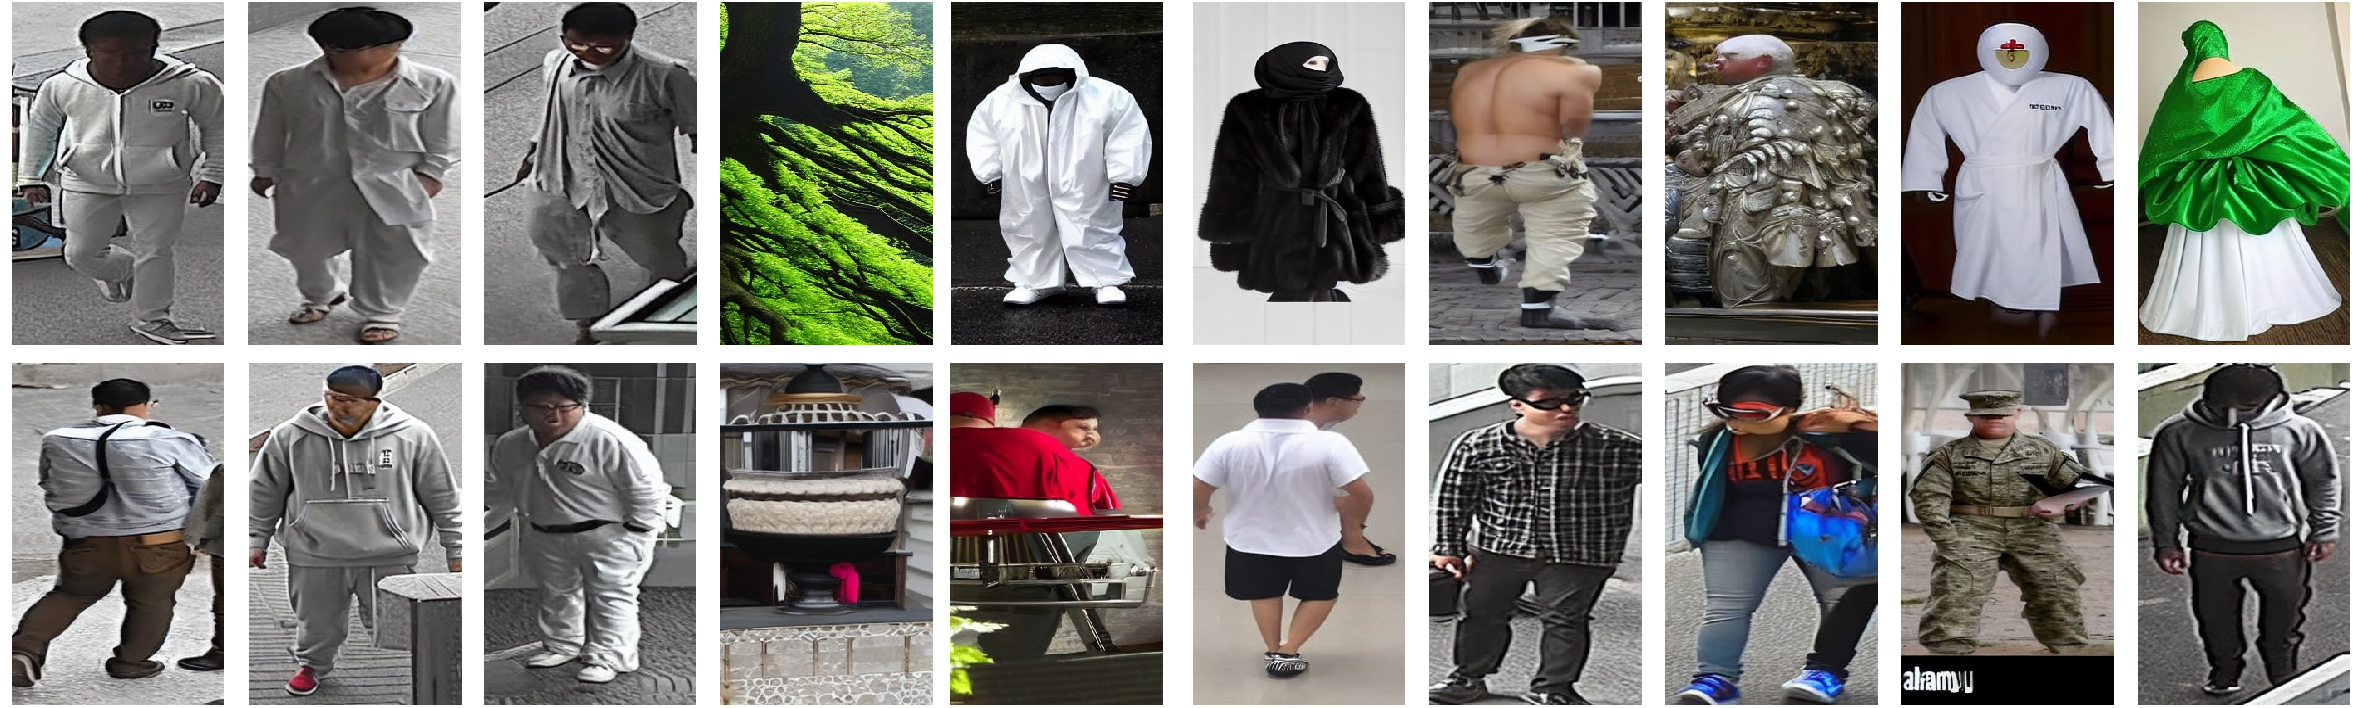
\includegraphics[width=1\linewidth]{images/bad.pdf}
\caption{The low-quality medium samples, generated by DaD, are mainly removed by 1) computing the file size and the mean variance of the difference between the 3 channels of every image; 2) OpenPose.
}
\label{fig: bad}
\end{figure}



